\chapter{Implementation}

\section{Deployment}

The whole solution is designed for and deployed in the Amazon Web Services (= AWS) cloud environment. It is a managed Virtual Private Cloud (= VPC) environment that is only accessible with company credentials and certificates.

\begin{figure}[!ht]
	\centering
	\includegraphics[width=0.8\textwidth]{figures/04_implementation/deployment_diagram}
    \caption{AWS System Architecture}
\end{figure}

\section{Issue Tracker}

The Issue Tracker used in my work environment is JIRA\footnote{No abbreviation here. It is short for GOJIRA, which is Godzilla in Japanese. Rumor has it that it is because the main competing product is Bugzilla.} by Atlassian. It is a standard project management tool providing bug tracking, issue tracking and many other functions. It is conveniently synergistic with other Atlassian tools such as Confluence (for documentation and wiki) and Bitbucket (formerly Stash), which is a server for version control (Mercurial and Git). The advantage is that all these three components are deployed in the AWS VPC environment. Thus, as a programmer I have fairly easy access to its internal APIs without being afraid to leak data where it shouldn't.

\subsection{API}

JIRA REST API is quite a mess, which is because Atlassian didn't develop all their products from scratch (Bitbucket was acquired) and it is still visible that the usage isn't seamless. In order to access Teams, Projects and Issues, two API endpoints have to be used:

\begin{enumerate}
	\item JIRA REST API
	\item JIRA REST AGILE
\end{enumerate}

Both of them are APIs (= Application Programming Interface), but I will use their names to distinguish one from another.Both are similar, but also slightly different from each other. 

To illustrate the subtle differences that drive any software engineer mad:

\begin{itemize}
	\item When JIRA REST API is used to obtain the issues, the resulting array uses pagination, because there could be a lot of issues and loading them all at once could take a significant amount of time. In order to determine whether the array I have is final, a parameter "total" is present in the response. This parameter tells how many issues in total there are. In order to load the whole list, it is necessary to keep track how many there are, and how many are left on the stack.
	
	\item When JIRA REST AGILE is used to obtain the teams, the resulting array also uses pagination. In order to determine whether the array I have is final, a parameter called "isLast" is present in the response, having, surprisingly, a boolean value true/false. Obviously, when the value is false, one has to load the next page with the last index that came before.
\end{itemize}

There are plenty of these little surprises that are so easily breakable with any update of the whole system. I honestly do not know, why it isn't the top priority for Atlassian to unite their APIs.

What struck me most though, is the absence of OAuth or Token-based communication. Every query is done via basic auth. While for development it is fine as it allowed me to quickly prototype on top of the API without the need to develop a complex token manager, for production it is quite inconvenient. Even though SSL certificates are all valid and in place, it simply is a terrible architectural choice to not have a proper way to authenticate other applications using the APIs.

\subsubsection{JQL}

JQL stands for JIRA Query Language \cite{jql}. It enables the API user to query the JIRA knowledge graph and extract information.

\begin{figure}[!ht]
	\centering
	
\includegraphics[width=0.5\textwidth]{figures/04_implementation/jql}
    \caption[JQL syntax]{JQL syntax (source~\protect\cite{jql})}
\end{figure}

\begin{enumerate}
	\item {\bf Field} - Fields are different types of information in the system. JIRA fields include priority, fixVersion, issue type, etc.
	\item {\bf Operator} - Operators are the heart of the query. They relate the field to the value. Common operators include equals (=), not equals (!=), less than (<), etc.
	\item {\bf Value} – Values are the actual data in the query. They are usually the item for which we are looking.
	\item {\bf Keyword} – Keywords are specific words in the language that have special meaning. In this post we will be focused on AND and OR.
\end{enumerate}

I used JQL in order to get all issues for a certain project:

\begin{lstlisting}
"https://jiraURL/issues/search?jql=project=SAUI"
\end{lstlisting}

Here I used simple query to search all issues where the project is SAUI (= Semantic Analysis of User Interactions). All URL encoders handle the double "= =" and it has never happened to me, that it would encode the parameters badly.

It can obviously be even more powerful, but I was glad it helped me easily get what I needed.

\subsubsection{Methods used}

All communication is handled via HTTP GET and all responses are in JSON format. Cross-site request forgery (= CSRF/XSRF) token system is disabled.

\begin{enumerate}
	\item To get all teams, method {\bf /board} has to be called on JIRA REST AGILE.
	\item To get all projects, method {\bf /projects} has to be called on JIRA REST API.
	\item To get all issues, method {\bf /search} with JQL query has to be called on JIRA REST API.
\end{enumerate}

Interestingly enough, even though, there are two API endpoints, the data is connected, so no further processing was necessary. It is important to note, that the responses are {\bf very} verbose and it is possible to tell in the query to the server not to send some fields back.

\subsection{DSL}

After a discussion with a UX lead, I came up with a simple solution - add keyword "WATCH:" on a new line and describe what to observe. Parsing is done line by line where the code searches the line for "WATCH:" (case insensitive) and extracts whatever follows until the end of line or occurrence of another "WATCH:". In order not to make it complex, end of line is the end of any description, it does not carry over to the next line.

\subsubsection{Examples}

Here are some examples how the parser for the DSL works. Validation of this technique will be covered in the Testing chapter.

\subsubsection*{Example 1 - Success}

\begin{lstlisting}
As a user, I want to be able to list all projects in the mobile app currently being tracked along with the number of tracked versions in the tracking system.

WATCH: Number projects expanded to the highest detail
WATCH: Filters used to extract information
\end{lstlisting}

This succeeds perfectly, as it parses everything without any hassle.

\subsubsection*{Example 2 - Success}

\begin{lstlisting}
As a user, I want to be able to list all projects in the mobile app currently being tracked along with the number of tracked versions in the tracking system. 
Watch:     Number projects expanded to the highest detail
Watch:     Filters used to extract information
\end{lstlisting}

This succeeds too, because the search is case insensitive and after the search, white spaces are extracted, so the result is the same as in the previous example.

\subsubsection*{Example 3 - Semi-success}

\begin{lstlisting}
As a user, I want to be able to list all projects in the mobile app currently being tracked along with the number of tracked versions in the tracking system.

WATCH: Number projects expanded to the highest detail, Filters used to extract information
\end{lstlisting}

This is a semi-success, almost a failure, but it still yields all the information that the user wanted. It just isn't nicely separated and would need some changes. The error is visible to the programmer and is easy to fix.

\subsubsection*{Example 4 - Failure}

\begin{lstlisting}
As a user, I want to be able to list all projects in the mobile app currently being tracked along with the number of tracked versions in the tracking system. WATCH: Number projects expanded to the highest detail. WATCH: Filters used to extract information
\end{lstlisting}

This yields only one result - "Number projects expanded to the highest detail.". While it seems like it is a good solution, the fact that it seems that way is unfortunately the worst thing about it - because it is hard to discover that there is an error. The programmer sees one observable action item and doesn't see that some got lost during the process, because it was all on one line.

\section{Semantic Data Manager}

The central part of the project should be robust and reliable. For that reason I chose Java as the main technology. For convenience and standardization of the code-base I opted for Spring Boot framework to help me with bootstrapping the heavy work (scheduling, threading, persistence etc.).

\begin{figure}[!ht]
	\centering
	\includegraphics[width=0.65\textwidth]{figures/04_implementation/sdm_deployment}
    \caption{Semantic Data Manager Deployment}
\end{figure}

Semantic Data Manager is deployed in AWS Elastic Beanstalk (= EB), which is Amazon's Platform as a Service (= PaaS) for Java web applications. It reduces management complexity without restricting choice or control. All it takes is to upload the application, and Elastic Beanstalk automatically handles the details of capacity provisioning, load balancing, scaling, and application health monitoring.

\newpage

\begin{figure}[!ht]
	\centering
	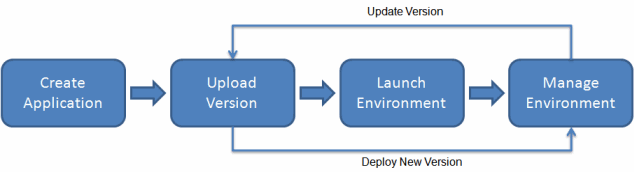
\includegraphics[width=0.5\textwidth]{figures/04_implementation/eb_flowchart}
    \caption[AWS Elastic Beanstalk Application Deployment]{AWS Elastic Beanstalk Application Deployment (source~\protect\cite{elasticbeanstalk})}
\end{figure}

It is important that the EB application runs in the same availability zone of the VPC as JIRA, otherwise it wouldn't be reachable at all.

The database runs on managed Amazon RDS (Relational Database Service), which is fast, secure and scalable deployment of database engine. It manages backups, software patching, automatic failure detection, and recovery. The default database engine is MySQL.

\subsection{Spring Boot}

I first tried to use play2 framework for educational purposes, but I encountered too many obstacles deploying play2 application to AWS: 

\begin{itemize}
	\item It does not support WAR packaging.\footnote{There is an unofficial tool that packages the code in a WAR file, but it is not recommended for production environment. Being constrained by highly regulated market, something that already says that it is not production ready is an instant "No thanks".}
	\item It is not possible to run play2 packages (packaged by Activator tool) on Tomcat Server.
	\item It comes with its own Netty Server, which is really clumsy to set up in AWS environment.
\end{itemize}

All three combined resulted in inability to synchronize the play2 application on port 9000 and NGINX running on port 5000. Unfortunately Netty Server does not support compile-time port configuration and NGINX does not support running Activator to set up the port during run-time, so I had to drop the idea of using play2 as I was simply unable to deploy the application. After researching and discussing with my peers and coworkers I looked up Spring MVC and stumbled upon Spring Boot, also recommended by my classmate. I tried few sample apps and found out it supports WAR packaging, runs natively on Tomcat and comes with almost the same perks like play2. I was ready to give it a try.

Primary goals of Spring Boot are:

"Spring Boot aims to make it easy to create Spring-powered, production-grade applications and services with minimum fuss. It takes an opinionated view of the Spring platform so that new and existing users can quickly get to the bits they need." \cite{spring-boot-blog}

\begin{itemize}
	\item Provide a radically faster and widely accessible getting started experience for all Spring development.
	\item Be opinionated out of the box, but get out of the way quickly as requirements start to diverge from the defaults.
	\item Provide a range of non-functional features that are common to large classes of projects (e.g. embedded servers, security, metrics, health checks, externalized configuration).
	\item Absolutely no code generation and no requirement for XML configuration.
\end{itemize}

\begin{figure}[!ht]
	\centering
	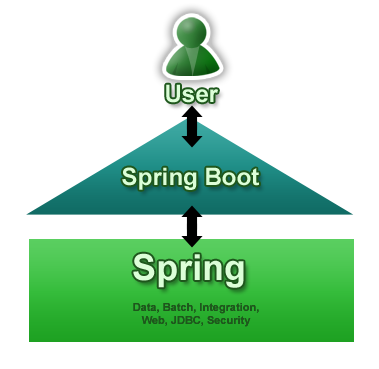
\includegraphics[width=0.4\textwidth]{figures/04_implementation/spring}
    \caption[Spring Boot architecture]{Spring Boot architecture (source~\protect\cite{spring-boot-doc})}
\end{figure}

The advantages seemed to be strong, development environment was convenient (native support in IntelliJ IDEA) and after some validation with Amazon support regarding AWS EB deployment in our VPC environment, I was confident this would be a good choice.

\subsection{Workflow}

The server makes the workflow very easy and exposes a REST API to obtain the information. Basic workflow is as follows:

\begin{enumerate}
	\item List available projects.
	\item List available issues in a project, along with parsed watched values.
	\item Prepare a configuration XML file (streamed as UTF8 encoded string) with selected issues.
\end{enumerate}

No registration, no other setup is necessary - it runs in the VPC environment, so only the employees can access it with their approved devices with the network certificates. Also, JIRA is open for everybody to read, so why bother with extra signing in/out and session management, if it's actually not desired. The component works as-is and serves only one purpose - to connect JIRA and the application code as easily as possible.

\newpage

\subsection{Technologies Used}

In order to make the development as comfortable as possible, I used various open-source frameworks/technologies to help me out with things that would otherwise take a lot of time.

\subsubsection{H2 Database}

H2 is a Java SQL database that I used in in-memory mode during the development (before switching to RDS). It is great for fast prototyping and validating of design ideas before using production database (RDS). Due to the fact that the entire database is deleted after a server is restarted, it enabled me to quickly change the schema without the need to do tedious database wipes. 

Another great thing is that it only needs to be defined in pom.xml and all other linking is provided out-of-the-box:

\bigbreak

\begin{lstlisting}
<dependency>
    <groupId>com.h2database</groupId>
    <artifactId>h2</artifactId>
</dependency>
\end{lstlisting}

Important note: as it wires up all connections automatically, it is absolutely vital not to have {\bf any other} database engine loaded via Maven, otherwise it crashes on start-up of Tomcat.

\subsubsection{Flyway}

Flyway is an open-source database migration tool. It aims to be clean and simple rather than robust and too complex. It uses 6 main commands:

\begin{enumerate}
	\item Migrate - Migrates the schema to the latest version.
	\item Clean - Drops all objects in the configured schemas.
	\item Info - Prints the details and status information about all the migrations.
	\item Validate - Validates the applied migrations against the available ones.
	\item Baseline - Baselines an existing database, excluding all migrations upto and including baselineVersion.
	\item Repair - Repairs the metadata table.
\end{enumerate}

Since I didn't need to migrate the database, thanks to the flexibility of H2, I mainly used Flyway for cold start (empty database). I defined, what will be in the database after the server has started and Flyway filled it up for me.

\newpage

\subsection{Code Deployment}

The code is packaged by Maven and deployed as a WAR file to AWS EB instance, running Tomcat 8 server. There is no need to configure anything with regards to basic networking - AWS EB is a back-to-back fully managed Platform as a Service (PaaS). Once deployed to VPC, the only thing that needs to be addressed is the availibility zone - making sure, it runs in the same zone as JIRA so they can communicate. It can be set up very quickly in the configuration section, however it can bring some frustration in the beginning when the developer doesn't know about it.

\bigbreak

There are multiple things to consider when deploying to AWS EB, even though it seems "super-easy" in most instructional videos and ads:

\begin{enumerate}
	\item Contrary to programmer's logic, one has to first create an "Application" and under that custom "Environments". In other words, Application is the main context, and environments are servers running in the same context, by default having the permission to communicate between each other.
	\item In Environment setup, we can choose either a Web Server Environment or a Worker Environment. Web Server is the hub of any application and is used in both Semantic Data Manager and Tracking Engine. Workers are only used in Tracking Engine and will be explained later.
	\item Chosen configuration was obviously Tomcat and I also opted for automatic load balancing and scaling.
	\item Opting to automatically create an RDS instance along with the environment is a really bad design. Once an environment is terminated, so is the database instance which causes a serious data loss.
	\item In order to access the servers via SSH, it is necessary to define a EC2 Security Group and assign it accordingly. Otherwise, all outside access is prohibited.
	\item It is also crucial to wisely choose the instance type. I opted for m3.medium, because Java applciations by themselves are quite demanding and I didn't want to risk being on the edge when strange errors occur because of insufficient memory capacity.
	\item Permissions and roles are absolutely crucial when it is desired to connect the Environment with other AWS services, such as object storage (S3 = Simple Storage Service) or a messaging queue (SQS = Simple Queue Service).
\end{enumerate}

 The size of the instance is recommended for any application running JVM. The configuration is Intel Xeon E5-2670 v2 (Ivy Bridge), 4GB SSD storage and 3.75GB RAM. Any additional memory is handled via S3.

\subsection{User Interface}

As mentioned before, Semantic Data Manager provides a REST API to be consumed by any kind of client capable of HTTP requests. Because my specialization are mobile applications, I chose to implement a mobile application for iOS as an administrating user interface for this component.

\subsubsection{Application Flow}

\begin{figure}[!ht]
	\centering
	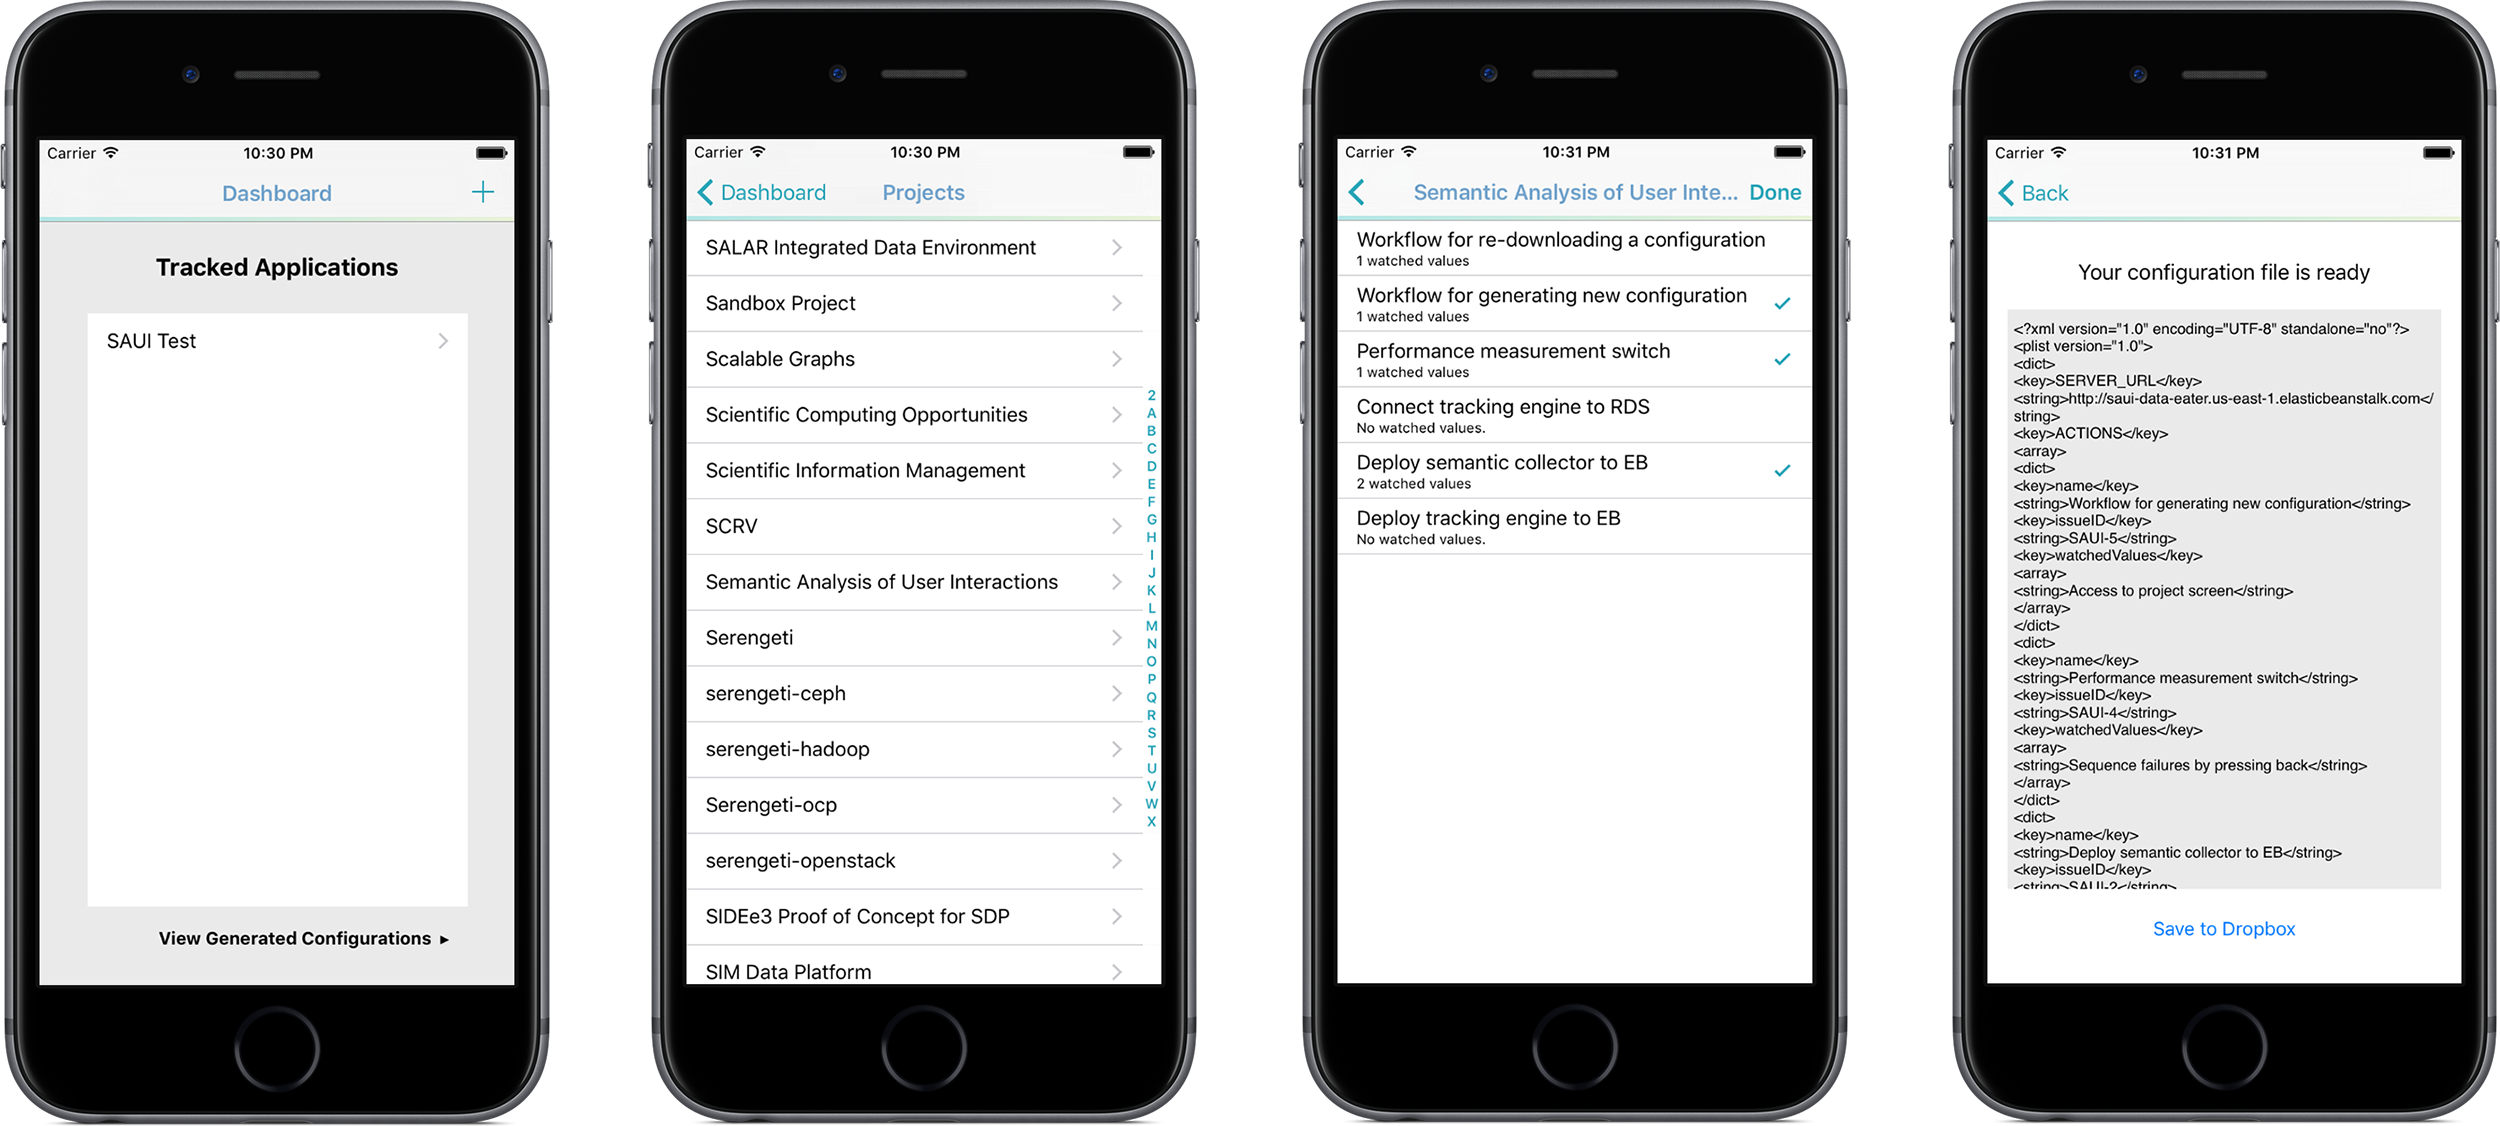
\includegraphics[width=0.95\textwidth]{figures/04_implementation/add_flow}
    \caption{Application Flow for Adding Configuration}
\end{figure}

\paragraph{Creating a new configuration}

\begin{itemize}
	\item First screen presents the user with currently tracked applications and two actionable items - add button and previously generated configurations. Add button leads to next step in order to generate a new configuration.
	\item Second screen has all available projects in a list, scrollable with alphabet index on the side. Naturally, selecting one, leads to the next step.
	\item The third screen shows all available issues along with their watched values. User is free to choose which one should be in the configuration (multiple-choice selection). When ready, the button "Done" proceeds with the process.
	\item The last screen shows the final configuration file that has been saved on the device. In order to send it to a computer, Dropbox integration has been implemented. When teams cooperate, it allows the user to automatically deliver the configuration file to all members of the team.
\end{itemize}

\newpage

\begin{figure}[!ht]
	\centering
	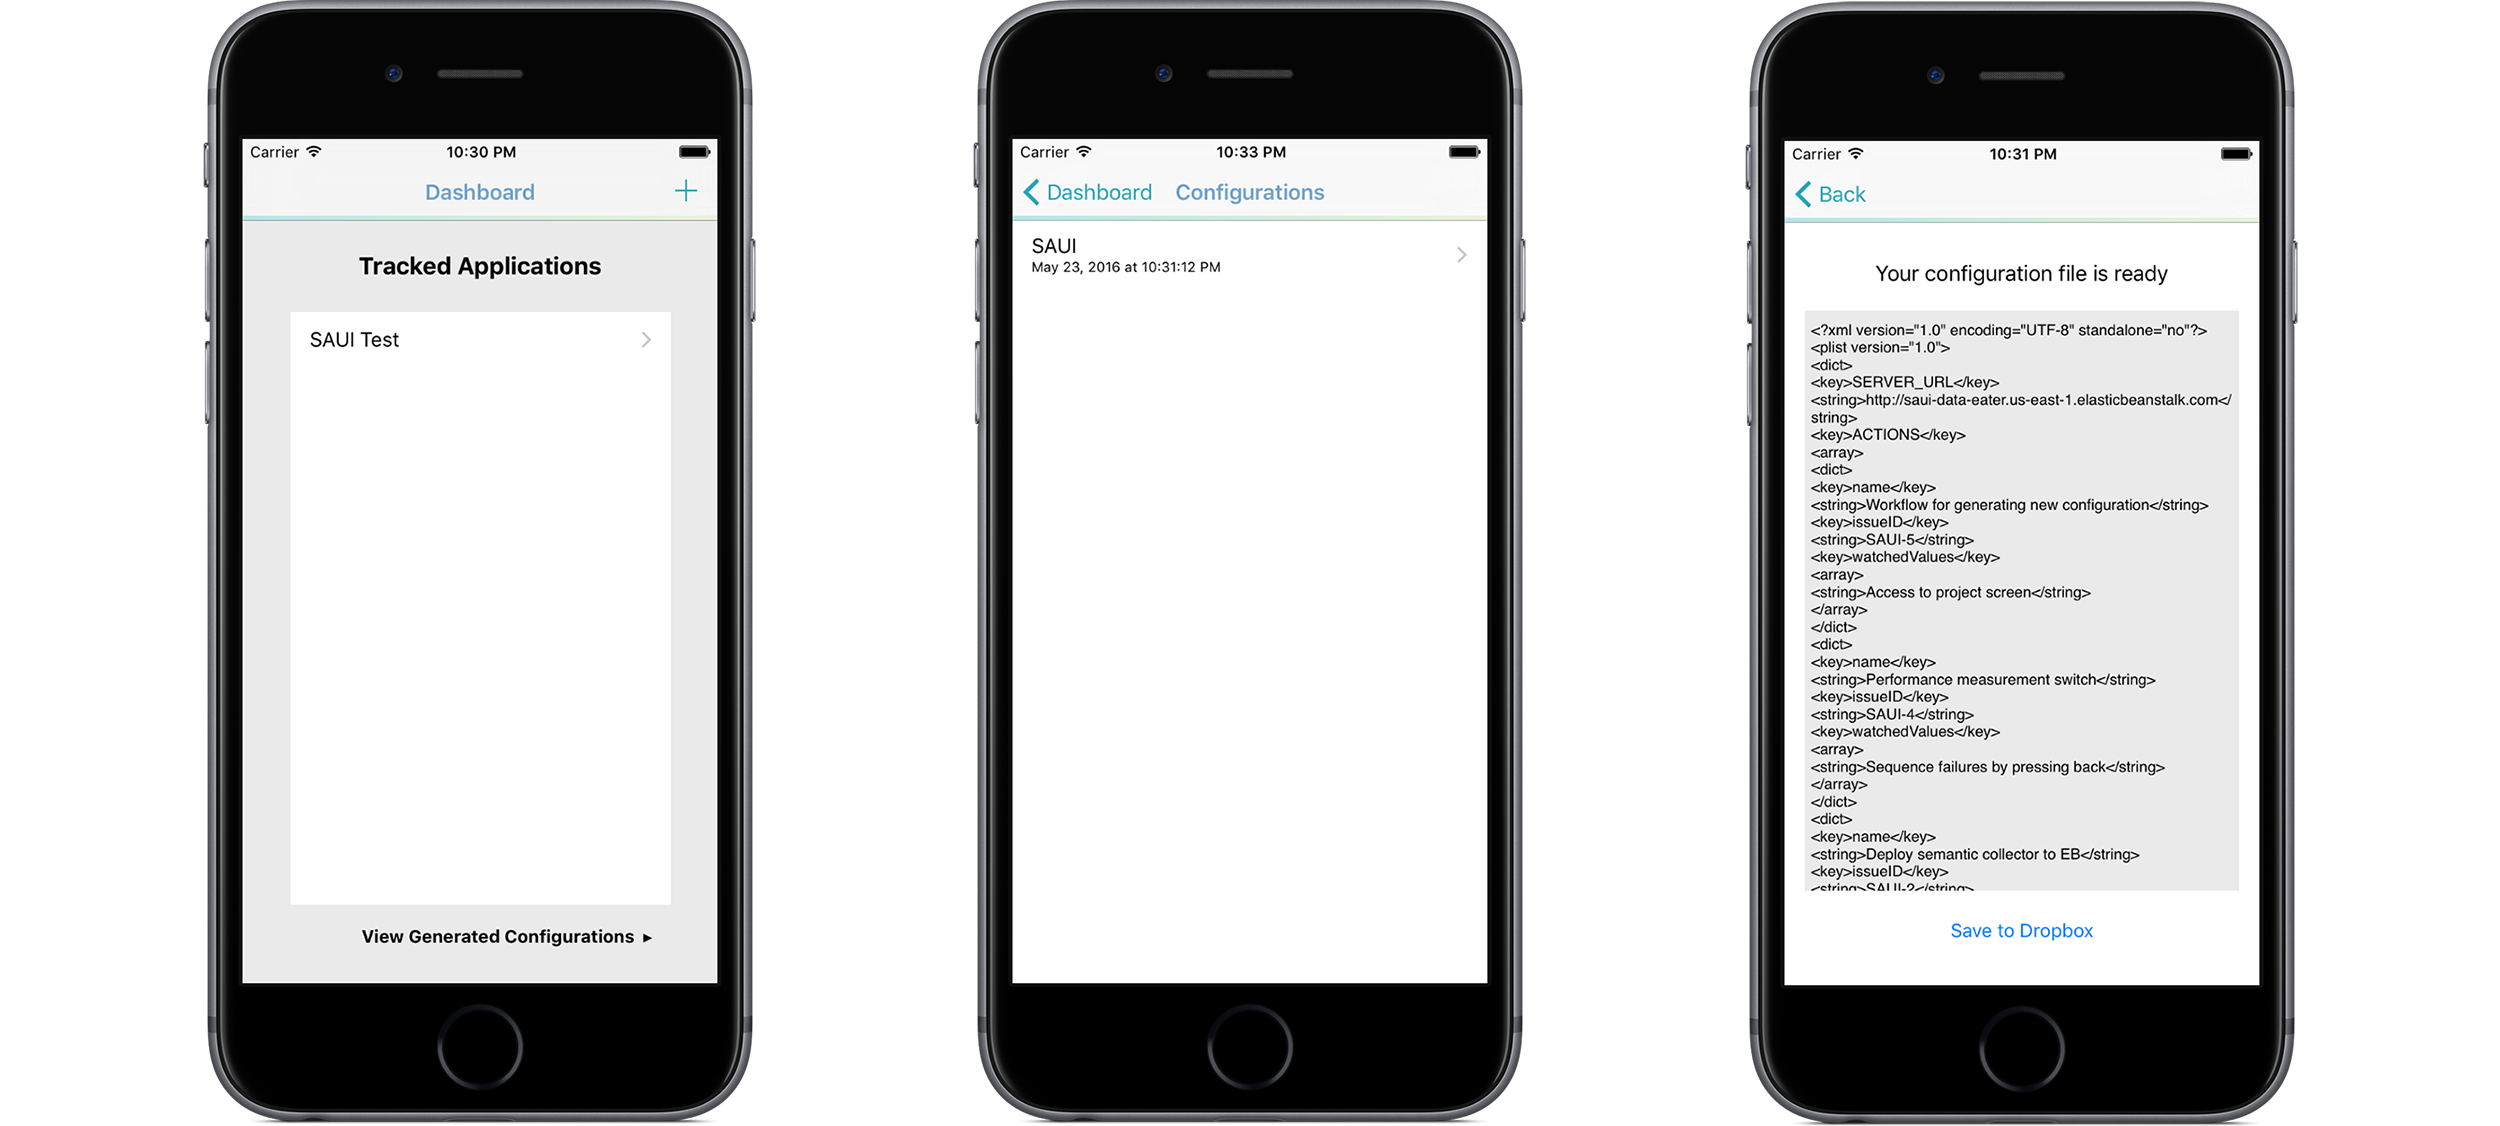
\includegraphics[width=0.95\textwidth]{figures/04_implementation/reconfig_flow}
    \caption{Application Flow for Recreating a Configuration}
\end{figure}

\paragraph{Recreating a previously generated configuration}

\begin{itemize}
	\item Instead of using the "Add" button the user proceeds with the "View Generated Configurations".
	\item Second screen shows previously generated configurations - those are immutable, because they are snapshots in time. They can only be re-downloaded again. If metadata has changed on JIRA, it is automatically updated.
	\item As the issue list is immutable in previously generated configurations, user is automatically redirected to the last screen with the generated configuration file.
\end{itemize}

\begin{figure}[!ht]
	\centering
	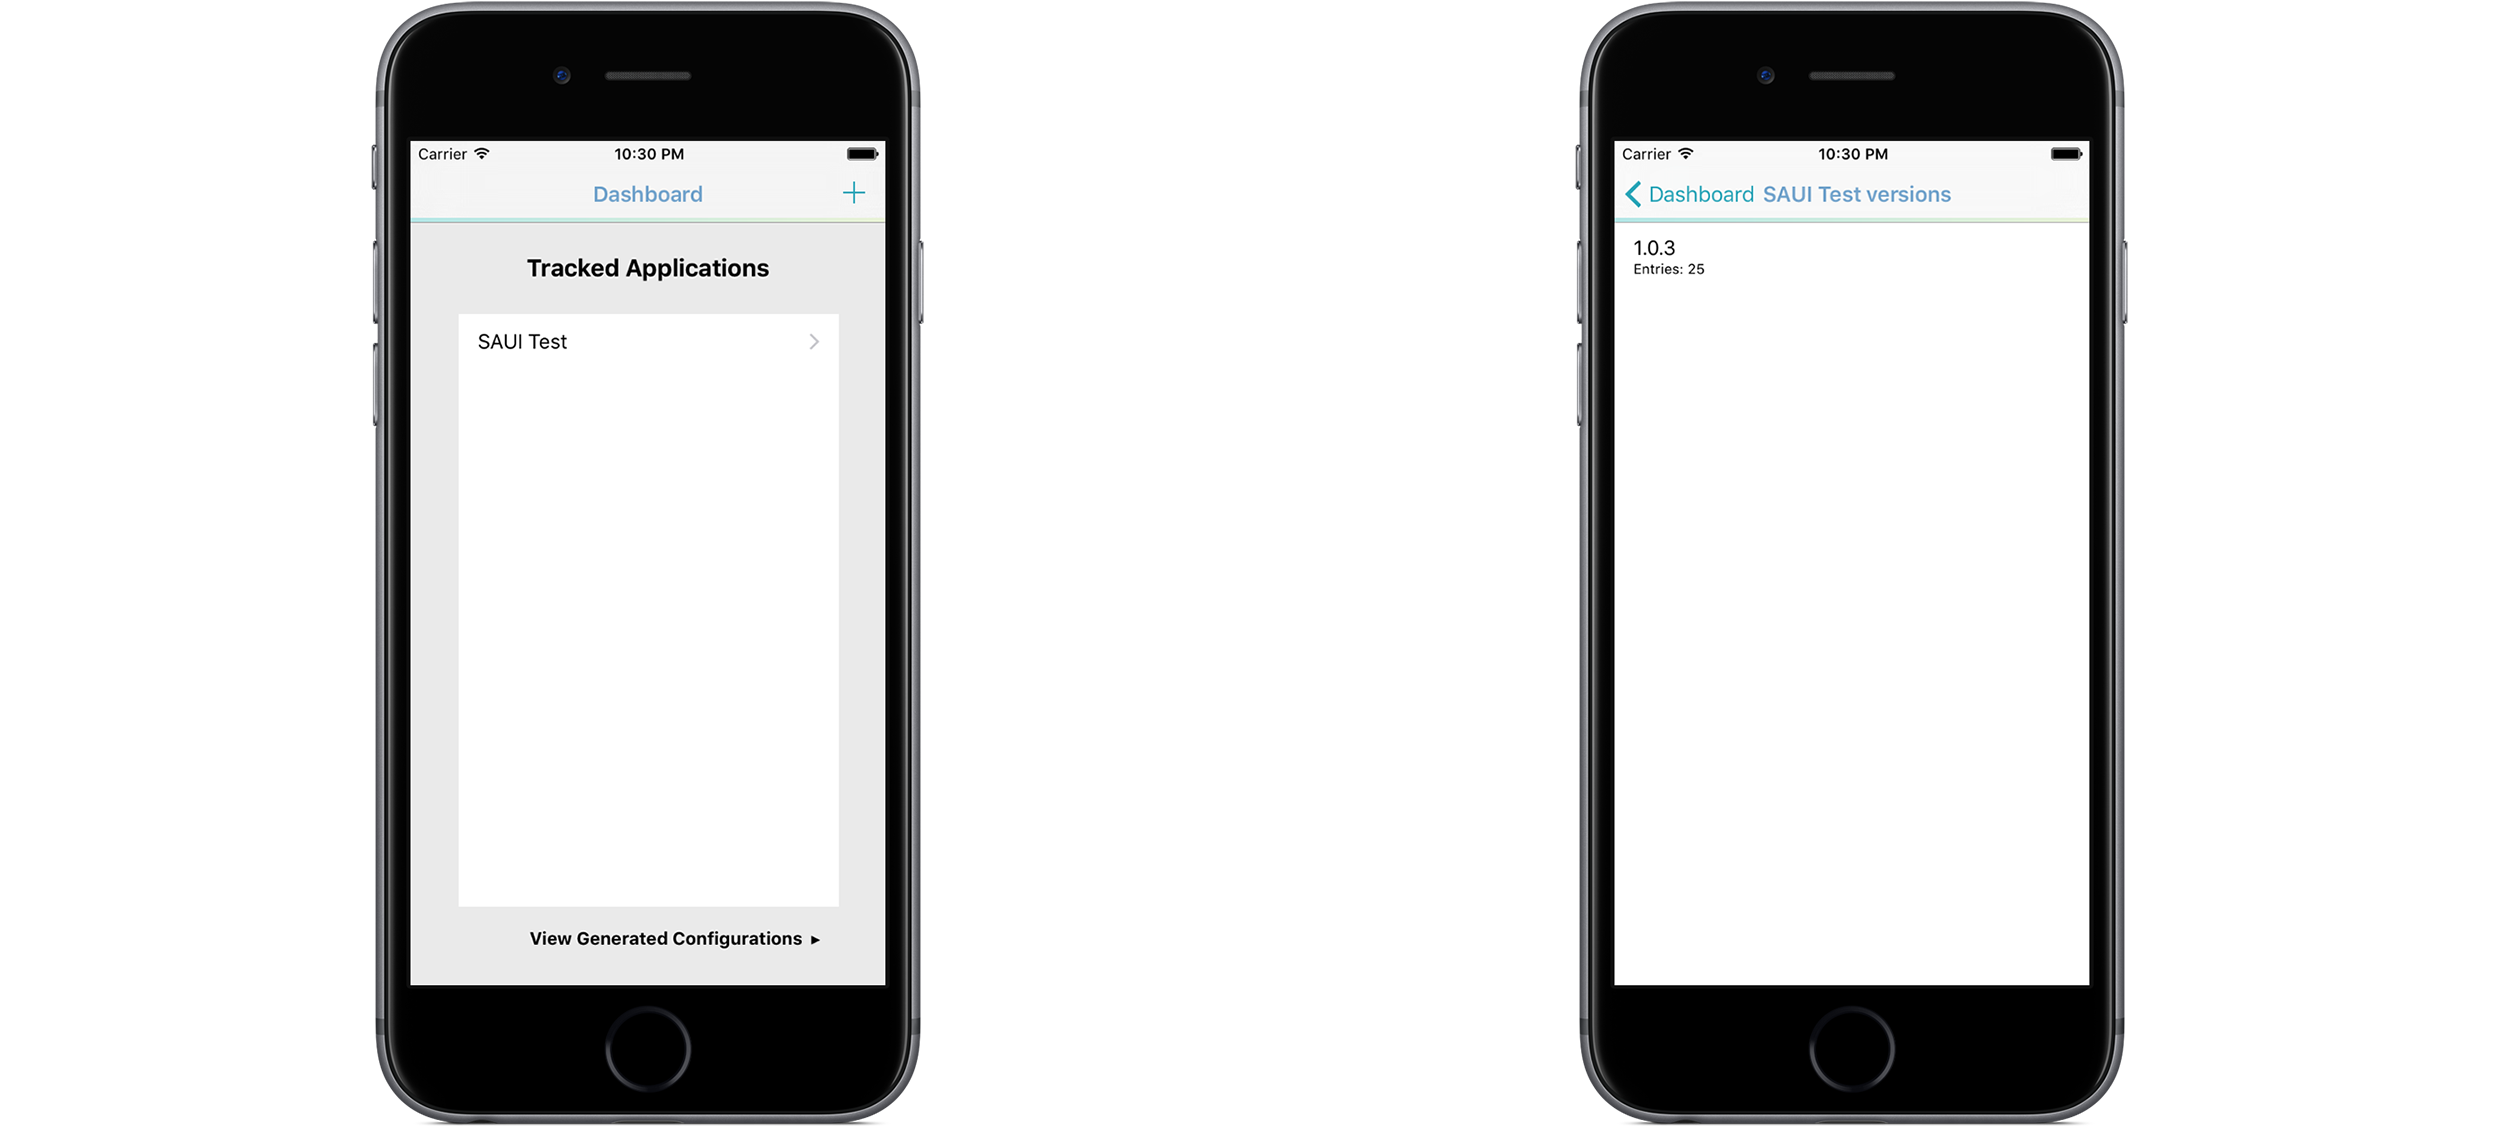
\includegraphics[width=0.95\textwidth]{figures/04_implementation/quick_summary}
    \caption{Application Flow for a Quick Overview of Gathered Data}
\end{figure}

\paragraph{Quick overview of gathered data}

\begin{itemize}
	\item Tapping on an application in the list of Tracked Applications leads to a quick overview of gathered data.
	\item The quick list of overview data is a simple list of the applications versions and number of entries for each version. This application doesn't serve as a statistical front-end, this screen only serves for quick overview for the user to know what's the current configuration status in the applications.
\end{itemize}

\subsubsection{Technologies Used}

\paragraph{Moya}\mbox{}\\
Moya\footnote{\url{https://github.com/Moya/Moya}} is an abstraction layer above an open-source networking library Alamofire\footnote{\url{https://github.com/Alamofire/Alamofire}}. It not only forces a cleaner code structure, but also makes it very well testable as it is a single gateway to the internet.

The main advantages are:

\begin{enumerate}
	\item Compile-time checking for correct API endpoint accesses.
	\item Ability to define a clear usage of different endpoints with associated enum values.
\end{enumerate}

\paragraph{SwiftyDropbox}\mbox{}\\
SwiftyDropbox\footnote{\url{https://github.com/dropbox/SwiftyDropbox}} is an official framework for iOS to integrate Dropbox functionality directly in the application. In order to use it, it is necessary to register the application in the Dropbox Developer Console. Personal usage requires no review by the Dropbox team, fully integrated one does. For the purposes of this thesis, the personal was sufficient.

\bigbreak

Both Moya and SwiftyDropbox are distributed via standard dependency management tool Cocoapods, which is a similar dependency tool like Maven or Gradle for Java. Written in Ruby, it is less verbose and therefore the dependency management file is fairly short (MBProgressHUD\footnote{\url{https://github.com/jdg/MBProgressHUD}} is a "loading" dialog when network operation is in process):

\bigbreak

\begin{lstlisting}
platform :ios, '9.0'
use_frameworks!

pod 'Moya'
pod 'SwiftyDropbox', '~> 3.0.0'
pod 'MBProgressHUD', '~> 0.9.1'
\end{lstlisting}

\newpage

\paragraph{Implementation Speciality}\mbox{}\\

Swift is a multi-paradigm language and allows the combination of object-oriented programming approach and functional programming approach. Because it was released in 2014 and doesn't have any legacy code carrying along, it has these features all built in. Along with proper generics and type safety rules. 

In one of the views (multiple-choice selection of issues), I had an interesting problem that I solved with the combination of the two mentioned paradigms. The situation was, that I had a list of immutable Issue objects representing the data displayed in the list. In order to keep track of which cells have been selected, I had to create another separate array containing boolean values, representing selected/unselected. This is important, ebcause the list view is dynamically generated and not keeping the record somewhere results in complete loss of selection on scroll, as the cells are generated as the user scrolls down/up. Unfortunately this results in having to perform manual filtering through the issues after the user is done selecting them. This is where the multi-paradigm comes in:

\bigbreak

\begin{lstlisting}
// declaration of properties - when issues are set after downloading, selectedIndicies is populated with false.

var selectedIndicies: [Bool] = []
var issues: [Dictionary<String, AnyObject>] = [] {
    didSet {
        selectedIndicies = [Bool](count:issues.count, repeatedValue: false)
    }
}

// filtering

let result = zip(self.issues, self.selectedIndicies).filter{$0.1}.map{$0.0}

// which the same as its longer version

let result2 = zip(self.issues, self.selectedIndicies)
	.filter{ (sequence: (object: Dictionary<String, AnyObject>, isSelected: Bool)) -> Bool in
		return object.isSelected
	}.map{ (filteredSequence: (object: String, isSelected: Bool)) -> String in
		return filteredSequence.object
	}


\end{lstlisting}

\bigbreak

This feature of the language is great, because it keeps the code clear and structured. There is absolutely no need for long and verbose code structures, using for cycles and being afraid that it might exceed the maximum index of an array. Also, the global functions on collections are better optimized by the compiler, resulting in 100\% speed increase of collection operations.\footnote{\url{http://stackoverflow.com/questions/29301577/performance-issue-while-finding-min-and-max-with-functional-approach/29305300\#29305300}}

\newpage

\section{Tracking Engine}

\begin{figure}[!ht]
	\centering
	\includegraphics[width=0.8\textwidth]{figures/04_implementation/tracking_diagram}
    \caption{Tracking Engine Diagram}
\end{figure}

Tracking Engine is also deployed in AWS EB but it its workflow is a bit more complex. The whole system is designed to be horizontally scalable on every component:

\begin{enumerate}
	\item {\bf Gateway} is scaled automatically by the Elastic Beanstalk environment.
	\item {\bf S3 and SQS} are scaled automatically by AWS.
	\item {\bf Aurora DB} is scaled automatically by AWS, along with replication and availability.
	\item {\bf Workers} are scaled automatically instance to instance (vertical scaling), or can be deployed multiple times as is necessary (horizontal scaling - in the console, simply choose "Clone Environment"). Sometimes it is cheaper to deploy more workers on less powerful instances instead of letting it scale automatically with just few.
\end{enumerate}

\subsection{Workflow}

The gateway is written in Java, also using the Spring-Boot framework. It's the main intersection for all the requests coming in an out. The workers are also another Spring-Boot application (deployed multiple times). Both of the applications use AWS SDK for connecting to S3 and the Aurora Database. The queue is implemented automatically in Amazon's environment and the only thing that a developer has to define is the method called on the worker (using HTTP POST). If the worker returns "200 OK", the message is considered as processed, so it is crucial to really throw an exception if one occurs, otherwise the message is lost.

\newpage

The general workflow is:

\begin{enumerate}
	\item When a client application sends in the stats of usage, it is designed to save as much data as possible - it is sent archived using GZIP\footnote{\url{http://www.gzip.org/}}. Because the data is serialized into a JSON file, GZIP performs really well and saves up to 70\% of data otherwise spent on sending the giant list of events.
	\item The gateway server takes the archive as it is and saves it to S3 object storage.
	\item After uploading the archive, the gateway server sends a message into the task queue SQS. The message is absolutely straight-forward containing only the name of the file. The name of the file is generated by the gateway server using the UUID library. If that's not enough, S3 makes sure there is never a collision in the names - if there is, it proposes a different name and returns it after the upload, so it's always unique.
	\item SQS then tries to deliver the message to an available worker. If it cannot be delivered it ends up "in flight", which is Amazon's implementation of dead letter queue. From there the Task queue system tries to deliver with a lowering frequency.
	\item When the message is delivered to the worker, it obtains the archive from S3, unzips it, parses and saves to the database. When done, it also removes the archive from S3. Then it confirms with "200 OK" marking that the message has been successfully processed.
\end{enumerate}

\subsection{Aurora Database}

Amazon Aurora is a fully managed, MySQL-compatible, relational database engine that combines the speed and reliability of high-end commercial databases with the simplicity and cost-effectiveness of open-source databases. It delivers up to five times the performance of MySQL.

\begin{figure}[!ht]
	\centering
	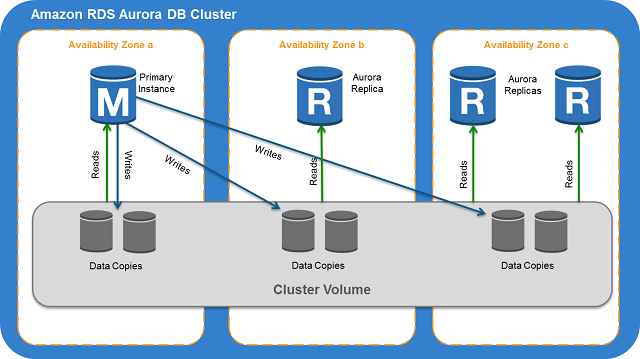
\includegraphics[width=0.6\textwidth]{figures/04_implementation/aurora}
    \caption[Aurora Replication Flow]{Aurora Replication Flow (source~\protect\cite{aurora})}
\end{figure}

\newpage

Every application operating with large volumes of data eventually one day runs into the wall having a bottleneck in the database. I decided not to compromise when I was choosing between the database engines. There was also a simple RDS instance available, just like the one I am using in the Semantic Data Manager, but this one will have exponentially more entries in the database then the Semantic Data Manager ever will.

Interestingly enough, Aurora DB wasn't officially supported by in the jdbc library enabling applications to connect to it. I managed to find it was in the Release Candidate 2 of the version 1.1.0 of the library. 

\bigbreak

\begin{lstlisting}
<dependency>
	<groupId>org.springframework.cloud</groupId>
	<artifactId>spring-cloud-aws-jdbc</artifactId>
	<version>1.1.0.RC2</version>
</dependency>
\end{lstlisting}

\bigbreak

The release of the official update is scheduled to June 2016.

\subsection{Deployment}

The networking capabilities of AWS are very broad and because the architecture of the Tracking Engine is quite complex, it is important to first introduce couple entities in the AWS cloud environment.

\subsubsection*{Identity and Access Management}

Identity and Access Management (= IAM) is a web service that allows the management of access to compute, storage, database and application services in the AWS cloud. It uses concepts known in other similar services in different environments - Users, Groups and Permissions. It is very detailed and allows specifications of which users have access to certain services, the kinds of actions they can perform and which resources are available (ranging from virtual machines, database instances and even the ability to filter database query results). Good thing is, that it works seamlessly with already existing identity management solutions, such as Active Directory\footnote{\url{https://technet.microsoft.com/en-us/library/dd448614.aspx}}

\subsubsection*{Permissions}

Permissions allow specifications of who has access to AWS resources, and what actions can be performed on those resources. Every IAM user starts with no permissions at all. In other words, by default, users can do nothing, not even view their own access keys. Permissions can be added to the user (attach a policy to the user) or the user can be assigned to a group that has the desired permissions.

Permissions can be assigned either as identity-based or as resource-based:

\begin{itemize}
	\item Identity-based, or IAM permissions are attached to an IAM user, group, or role and allow specification of what that user, group, or role can do.
	\item Resource-based permissions are attached to a resource. Resource-based permissions allow specification of who has access to the resource (S3, SQS) and what actions they can perform on it. Resource-based policies are inline only, not managed.
\end{itemize}

\subsubsection*{Policies}

To assign permissions to a user, group, role, or resource, a policy has to be created. Policy is a document that explicitly lists permissions.

Policy allows specification of the following:

\begin{itemize}
	\item Actions: which actions should be allowed. Every service has its own set of actions.
	\item Resources: which resources should be allowed to perform actions on.
	\item Effect: which effect will a request to access by a user - deny or allow.
\end{itemize}

All policies are defined by a JSON file and can be assigned in totally granular fashion to every service and user.


\subsubsection*{Security Group}

A security group acts as a virtual firewall that controls the traffic for one or more instances. When an instance is launched, it can be associated with one or more security groups. Each group has rules that can be added that allow traffic to or from its associated instances. All rules for a security group can be modified at any time. The new rules are automatically applied to all instances that are associated with the security group. When a decision has to be made whether to allow traffic to reach an instance, all the rules from all the security groups associated with the instance are evaluated.

\bigbreak

The whole AWS cloud environment is very complex and has way more to offer than just the couple points I listed above. For the sake of deploying my architecture it is sufficient. For anything else, AWS documentation\footnote{\url{http://docs.aws.amazon.com/IAM/latest/UserGuide/introduction.html}} is of very high quality and virtually any question can be answered there.

\newpage

Having the knowledge of all necessary foundations of the inner workflow in AWS, all of these prerequisites have to be met in order to deploy the Tracking Engine:

\begin{enumerate}
	\item AWS EB application with IAM role with permissions to access SQS and S3.
	\item Policy on S3 for the IAM role set up to be able to read/write via JSON configuration:
	
\begin{lstlisting}
"Statement": [
		{
			"Sid": "sid123456789",
			"Effect": "Allow",
			"Principal": "*",
			"Action": "s3:*",
			"Resource": [
				"arn:aws:s3:::iam-role-name/*",
				"arn:aws:s3:::iam-role-name"
			]
		}
	]
\end{lstlisting}	
	
	\item Aurora Database instance up and running with the same Security Group as the AWS EB application.
	\item Open 3306 port in the Security Group between the AWS EB application and the Aurora Database.
\end{enumerate}

Everything else is automatic when the AWS EB application is set up as described with the Semantic Data Manager. Database URL is for security reasons injected through environment variables (it should never be hard-coded!).

\subsection{Timeseries Application}

The administration application for the Semantic Data Manager does provide a quick overview, but that is not meant to serve as a dashboard or any decision-making helper tool. It's merely just a peak on whether or not the desired application version is being tracked. Clearly that is not optimal for deriving any conclusions.

In order to show the power of the gathered data I developed another mobile application meant just for displaying the flow of the data in time. It is inspired by the popular application Numerous\footnote{\url{http://numerousapp.com/}}, available on the Apple App Store.

The requirements for such an applications could be endless - graph mash-ups, benchmarking and so much more. In order to simply demonstrate the movement in the KPIs and the potential in the data, I chose to display the total increase/decrease of entries during the last 5 days.

\newpage

\begin{figure}[!ht]
	\centering
	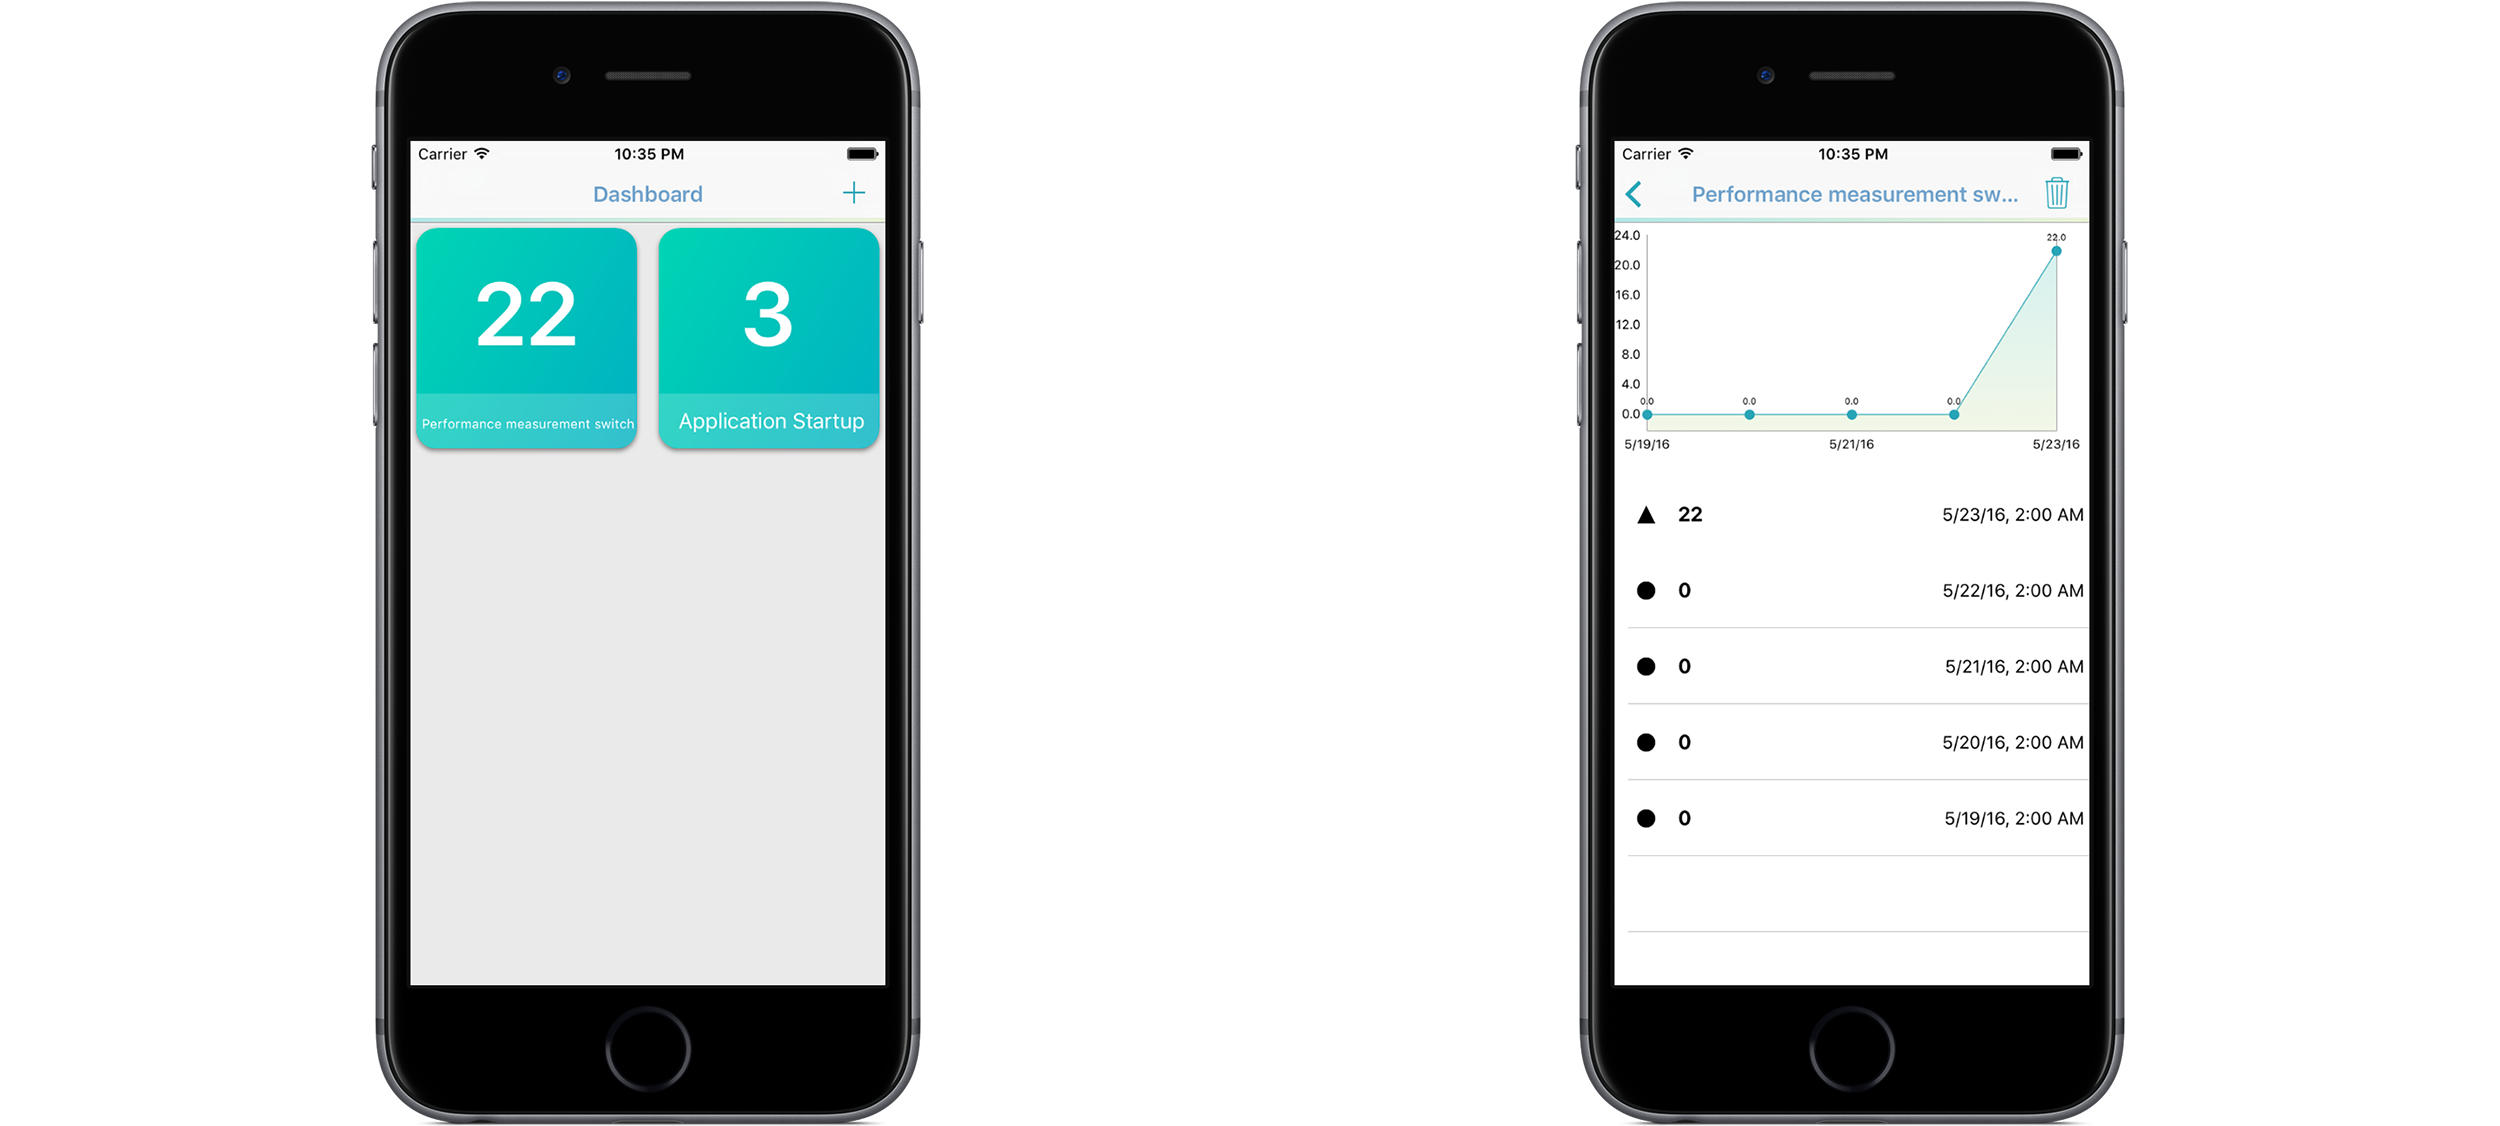
\includegraphics[width=0.95\textwidth]{figures/04_implementation/time_flow}
    \caption{Time Series Detail}
\end{figure}

\begin{enumerate}
	\item After choosing an application through the "Add" button (the list looks identical to any previous lists), the application automatically loads all KPIs available on the server. The number marks the total number of entries in the last 5 days.
	\item By tapping on a number in the grid, a detailed graph is displayed having total number of entries per day - summing up to the same number as is displayed on the dashboard. The KPI can be deleted from the application so it's not displayed anymore (it remains on the server), because the application persists what was selected in the choice of applications and refreshes it on the next start of the application.
\end{enumerate}

\subsubsection{Technologies Used}

Aside from the technologies already listed in the administration application (which I have used again) - Moya and MBProgressHUD, I also used:

\paragraph{ios-charts}\mbox{}\\

ios-charts is a charting library based on MPAndroidChart\footnote{\url{https://github.com/danielgindi/Charts}}. It is written in Swift and supports plethora of chart types - line charts, bar charts, pie charts, scatter plots, box plots, bubble charts and radar charts.

The setup is quite "procedural" and requires a lot of boilerplate code, but when it's well set up, the result is very satisfying.

\newpage

\paragraph{Realm.io Database}\mbox{}\\

Realm is a mobile database made by a start-up of the same name. Developed by two engineers from Nokia - Alexander Stigsen and Bjarne Christiansen, it is currently one of the most used frameworks used for iOS development. 

The main advantages are:

\begin{itemize}
	\item Mobile-first: built from the ground up to run directly inside phones, tablets and wearables.
	\item Simple: Data is directly exposed as objects and queryable by code.
	\item Fast: Realm is faster than SQLite on common operations.
\end{itemize}

The great thing in comparison to CoreData, a native Apple framework on top of SQLite, is not having to keep the context object everywhere, where a anything can be written in the database. Another great tool shipped with the framework is a migration tool, that has a similar philosophy to Flyway described before.

\subsubsection{API used}

Obviously, the goal is to send the data in as condensed format as possible. For those reasons, the automatically exposed API by Spring-Boot was too verbose. In order to load the data, I created another Controller endpoint in the Tracking Engine application that those handles special requests from the Timeseries application:

\begin{enumerate}
	\item \emph{/mobile/applicationEntryTypes} - returns a list of all KPIs in an application.
	
\begin{lstlisting}
{ "entryTypes" : [
		{"applicationName":"SAUI Test","applicationVersion":"1.0.3","name":"Performance measurement switch","total":12654}
	]
}	
\end{lstlisting}	
	
	\item \emph{/mobile/applicationEntrySummary} - returns 5 day entry count for a given KPI.
	
\begin{lstlisting}
{ "entries":[ ... ],
  "metadata":[
		{"entries":11,"timestamp":1464048000}, ...
	]
}
\end{lstlisting}	
\end{enumerate}

\newpage

\section{Tracked Device SDK}

In order to integrate the domain vocabulary generated by the Semantic Data Manager, it is necessary to have an interpreter of such vocabulary. For the implementation for Apple devices, I chose native development in Swift.

As stated in the previous chapter, the SDK has two layers - the configuration interpreter and an interface to log an event.

\subsection{Interpreter}

The interpreter enables the storing interface to call functions on it that extract the information from the configuration file, without the need to handle the low-level file access. It is made to be as precise as possible - no errors allowed. When the configuration file is not present it calls a system level fatalError function. 

Methods exposed:

\begin{itemize}
	\item \emph{getDictionary} - returns the whole configuration file as a dictionary object
	\item \emph{getURL} - returns the URL of the Tracking Engine
	\item \emph{getAllActions} - returns all actions available in the dictionary
\end{itemize}

\subsection{Interface for storing}

The interface for storing provides couple functions:

\begin{enumerate}
	\item \emph{startEvent(itemIndex: Int)} - logs beginning of an event on the given index in the configuration.
	\item \emph{finishEvent(itemIndex: Int)} - logs the end of an event on the given index in the configuration.
	\item \emph{watchValue(itemIndex: Int, valueIndex: Int)} - logs an action of watched value on the given index assigned to an event on the given index in the configuration.
	\item \emph{reportData(compressed: Bool, success: (() -> Void)?)} - reports data to the server, either in compressed format or not and after finishing it calls the optional (not mandatory to use) completion closure.
\end{enumerate}

If an event is to be logged and the interpreter doesn't find it, fatalError is called again.

\newpage

To ensure clean code and the level of "security"\footnote{Security here refers to the Defensive Programming coding style leading to reduced number of bugs and problems.} of the code Swift's if-let and guard statements came in very handy:

\bigbreak

\begin{lstlisting}
func startEvent(itemIndex: Int) {
	guard let action = ConfigurationReader.getAllActions()[safe: itemIndex]
		else {
			fatalError("Action at given index (\(itemIndex)) does not exist!")
	}
        
	if let name = action["name"] as? String, issueID = action["issueID"] as? String {
		self.addEvent("START", name: name, issueID: issueID)
	} else {
		fatalError("Action at given index (\(itemIndex)) has details in wrong format!")
	}
}
\end{lstlisting}	

\bigbreak

The guard statement and the if-let statement are somewhat similar - they make sure that an object the developer is trying to access is not null and will not cause any problems. The main difference is that if-let goes inside curly brackets and creates more complexity by indented code. Guard statement allows in-line handling, however it does not allow chaining of the statements, like the if-let statement does.

In fact, even more interesting feature is used in the code snippet above - Swift extension. The safe look-up of an action in the array of all actions is a separate function written as an extension to the standard collection functions in Swift. The extension is written this way:

\bigbreak

\begin{lstlisting}
extension Array {
    subscript (safe index: Int) -> Element? {
        return indices ~= index ? self[index] : nil
    }
}
\end{lstlisting}	

\bigbreak

There is no need to override the whole Array object and implement a new method. The compiler takes it as a new first-class function on the collection and it can be used in the whole project.

\newpage

\subsection{Distribution}

When a developer wants to use an external library, there are two standard ways how to get it to the project:

\begin{enumerate}
	\item Cocoapods
	\item Carthage
\end{enumerate}

Cocoapods is more invasive - it links the source code into the project as another sub-targets and creates a new workspace for Xcode. Sometimes it can be frustrating, especially during clean builds when having more than 5 dependencies can take 5 minutes or more to fully compile.

Carthage is a non-invasive way of importing dependencies, however it is not standardized by Apple - it requires initial setup in Xcode and is subject to break during Xcode updates.

\bigbreak

Requirements were to create both, which is creating a Podspec file for Cocoapods and a Cart file for Carthage:

\begin{lstlisting}
// Cartfile
github "Moya/Moya" ~> 6.4.0
github "realm/realm-cocoa" ~> 0.99
github "nicklockwood/GZIP" ~> 1.1

//Podspec
Pod::Spec.new do |s|
  s.name         = "SAUI"
  s.version      = "1.0"
  s.summary      = "Network abstraction layer written in Swift"
  s.author             = { "Michal Svacha" => "svachmic@fel.cvut.cz" }
  s.ios.deployment_target = '8.0'
  s.osx.deployment_target = '10.9'
  s.watchos.deployment_target = '2.0'
  s.tvos.deployment_target = '9.0'
  s.source       = { :git => "https://url/SAUI.git", :tag => s.version }
  s.default_subspec = "Core"

  s.subspec "Core" do |ss|
    ss.source_files  = "Source/*.swift", "Source/Plugins/*swift"
    ss.dependency "Moya", "~> 6.4.0"
    ss.dependency "RealmSwift", "~> 0.99"
    ss.dependency "GZIP", "~> 1.1"
    ss.framework  = "Foundation"
  end
end

\end{lstlisting}	

\newpage

\subsection{Workflow}

The usage of the framework after linking is very straight forward. The main object to use is called \emph{Reporter} - it is singleton and accessible via it's proeprty \emph{sharedInstance}. The Reporter class is the interface for storing and offers all methods listed in previous section.

It can be initially set up whether the reporting to the server will be handled automatically or not. If not, the developer has to handle the upload scheduling himself and call the function \emph{reportData} whenever needed. If the automatic reporting is set up, an NSTimer thread object runs in the background, firing every 120 seconds to check if there is anything in the database to be reported. If yes, it gets uploaded to the server.

\subsection{Technologies Used}

Aside from all the technologies previously listed - Moya and Realm, in this component I had to also use Alamofire from which I tried to abstract myself away with Moya. Unfortunately Moya does not support uploading binary data via POST, so I had to use a lower-level tool to get the archived data to the server.

Another technology I used here is a GZIP library handling the archiving of data. The library comes with a choice of level of encryption, which for a text can be naturally selected to the highest number. The object that is archived can only be an NSData object, so I serialized the JSON that is supposed to be archived into UTF8-encoded data:

\bigbreak

\begin{lstlisting}
let jsonData = try! NSJSONSerialization.dataWithJSONObject(events, options: NSJSONWritingOptions.PrettyPrinted)
let archived = jsonData.gzippedDataWithCompressionLevel(1.0)!
\end{lstlisting}	
